\section{\lego\ Implementation}
\label{sec:lego:impl}

We implemented \lego\ in C on the x86-64 architecture.
\lego\ can run on commodity, off-the-shelf machines 
and support most commonly-used Linux system call APIs.
Apart from being a proof-of-concept of the \splitkernel\ OS architecture,
our current \lego\ implementation can also be used on existing datacenter servers to reduce the energy cost,
with the help of techniques like Zombieland~\cite{Nitu18-EUROSYS}.
Currently, \lego\ has 206K SLOC,
with 56K SLOC for drivers.
\lego\ supports 113 syscalls, 15 pseudo-files,
and 10 vectored syscall opcodes. 
Similar to the findings in ~\cite{tsai-eurosys16}, we found that implementing these Linux interfaces
are sufficient to run many unmodified datacenter applications.

\subsection{Hardware Emulation}
Since there is no real resource disaggregation hardware,
we emulate disaggregated hardware components using commodity servers 
by limiting their internal hardware usages.
For example, to emulate controllers for \mcomponent{}s and \scomponent{}s, 
we limit the usable cores of a server to two.
To emulate \pcomponent{}s, we limit the amount of usable main memory of a server
and configure it as \lego\ software-managed \excache.

\subsection{Network Stack}
We implemented three network stacks in \lego.
The first is a customized RDMA-based RPC framework we implemented based on LITE~\cite{Tsai17-SOSP}
on top of the Mellanox mlx4 InfiniBand driver we ported from Linux.
Our RDMA RPC implementation registers physical memory addresses with RDMA NICs 
and thus eliminates the need for NICs to cache physical-to-virtual memory address mappings~\cite{Tsai17-SOSP}.
The resulting smaller NIC SRAM can largely reduce the monetary cost of NICs,
further saving the total cost of a \lego\ cluster.
All \lego\ internal communications use this RPC framework.
For best latency, we use one dedicated polling thread at RPC server side to keep polling incoming requests.
Other thread(s) (which we call worker threads) execute the actual RPC functions. 
For each pair of components, we use one physically consecutive memory region at a component
to serve as the receive buffer for RPC requests. 
The RPC client component uses RDMA write with immediate value to directly write 
into the memory region and the polling thread polls for the immediate value to get the metadata 
information about the RPC request (\eg, where the request is written to in the memory region).
Immediately after getting an incoming request, the polling thread passes it along to a 
work queue and continues to poll for the next incoming request.
Each worker thread checks if the work queue is not empty and if so, gets an RPC request 
to process. Once it finishes the RPC function, it sends the return value back to the RPC client 
with an RDMA write to a memory address at the RPC client.
The RPC client allocates this memory address for the return value before sending the RPC request
and piggy-backs the memory address with the RPC request.

The second network stack is our own implementation of the socket interface directly on RDMA.
The final stack is a traditional socket TCP/IP stack we adapted from lwip~\cite{lwip} 
on our ported e1000 Ethernet driver.
Applications can choose between these two socket implementations 
and use virtual IPs for their socket communication.

\subsection{Processor Monitor}
\label{sec:lego:procimpl}

We reserve a contiguous physical memory region during kernel boot time
and use fixed ranges of memory in this region as \excache, tags and metadata for these caches, and kernel physical memory. 
We organize \excache\ into virtually indexed sets with a configurable set associativity.
Since x86 (and most other architectures) uses hardware-managed TLB and walks page table directly after TLB misses, 
we have to use paging and the only chance we can trap to OS is at page fault time. 
We thus use paged memory to emulate \excache, 
with each \excache\ line being a 4\KB\ page.
A smaller \excache\ line size would improve the performance of fetching lines from \mcomponent{}s
but increase the size of \excache\ tag array and the overhead of tag comparison. 

An \excache\ miss causes a page fault and traps to \lego.
To minimize the overhead of context switches,
we use the application thread that faults on a \excache\ miss
to perform \excache\ replacement.
Specifically, this thread will identify the set to insert the missing page
using its virtual memory address,
evict a page in this set if it is full,
and if needed, flush a dirty page to \mcomponent\ 
(via a \lego\ RPC call to the owner \mcomponent\ of the \vregion\ this page is in).
To minimize the network round trip needed to complete a \excache\ miss,
we piggy-back the request of dirty page flush and new page fetching
in one RPC call when the \mcomponent\ to be flushed to and the \mcomponent\ to fetch the missing page are the same.

\lego\ maintains an approximate LRU list for each \excache\ set 
and uses a background thread to sweep all entries in \excache\ and adjust LRU lists.
\lego\ supports two \excache\ replacement policies:
FIFO and LRU. For FIFO replacement, we simply maintain a FIFO queue for each \excache\ set and insert a
corresponding entry to the tail of the FIFO queue when
an \excache\ page is inserted into the set. Eviction victim is chosen as the head of the FIFO queue. 
For LRU, we use one background thread to sweep all sets of \excache\ to adjust their LRU lists.
For both policies, we use a per-set lock and lock the FIFO queue (or the LRU list) when
making changes to them.

\subsection{Memory Monitor}
\label{sec:lego:memimpl}

We use regular machines to emulate \mcomponent{}s 
by limiting usable cores to a small number (2 to 5 depending on configuration).
We dedicate one core to busy poll network requests 
and the rest for performing memory functionalities. 
The \lego\ memory \microos\ performs all its functionalities as handlers of RPC requests from \pcomponent{}s.
The memory \microos\ handles most of these functionalities locally
and sends another RPC request to a \scomponent{} for storage-related functionalities (\eg, when a buffer cache miss happens).
\lego\ stores application data, application memory address mappings, vma trees, and \vregion\ arrays
all in the main memory of the emulating machine. 
%from application process virtual memory addresses to 
%local physical memory addresses.

The memory \microos\ loads an application executable from \scomponent{}s 
to the \mcomponent, handles application virtual memory address allocation requests,
allocates physical memory at the \mcomponent,
and reads/writes data to the \mcomponent.
Our current implementation of memory \microos\ is purely in software,
and we use hash tables to implement the virtual-to-physical address mappings.
While we envision future \mcomponent{}s to implement memory \microos{}s in hardware and
to have specialized hardware parts to store address mappings,
our current software implementation can still be useful for 
users that want to build software-managed \mcomponent{}s.

\subsection{Storage Monitor}
Since storage is not the focus of the current version of \lego,
we chose a simple implementation of building storage \microos\ on top of the Linux {\em vfs} layer as a loadable Linux kernel module.
\lego\ creates a normal file over vfs as the mount partition for each \vnode\
and issues vfs file operations to perform \lego\ storage I/Os.
Doing so is sufficient to evaluate \lego, while largely saving our implementation efforts on storage device drivers and layered storage protocols.
We leave exploring other options of building \lego\ storage \microos\ to future work.

{
\begin{figure*}[th]
\begin{center}
\centerline{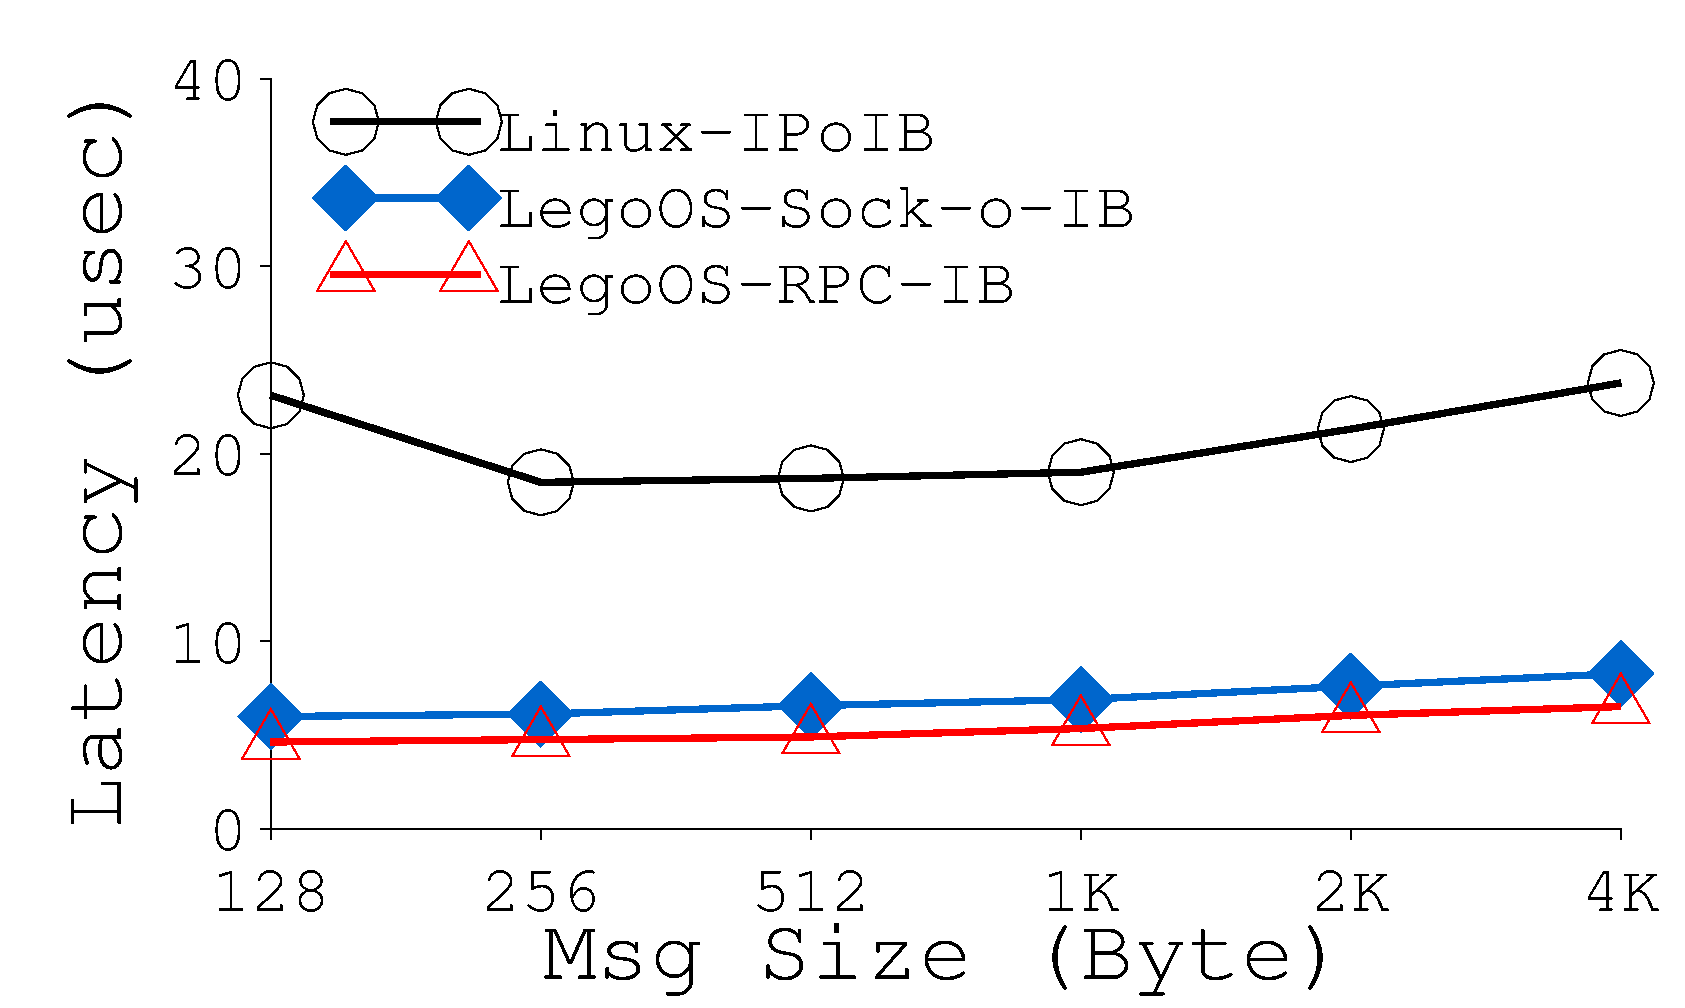
\includegraphics[width=0.5\textwidth]{lego/Figures/g_plot_LEGO_latency.pdf}}
\caption[Network Latency.]{Network Latency.}
\label{fig-net-latency}
\end{center}
\end{figure*}
}
{
\begin{figure*}[th]
\begin{center}
\centerline{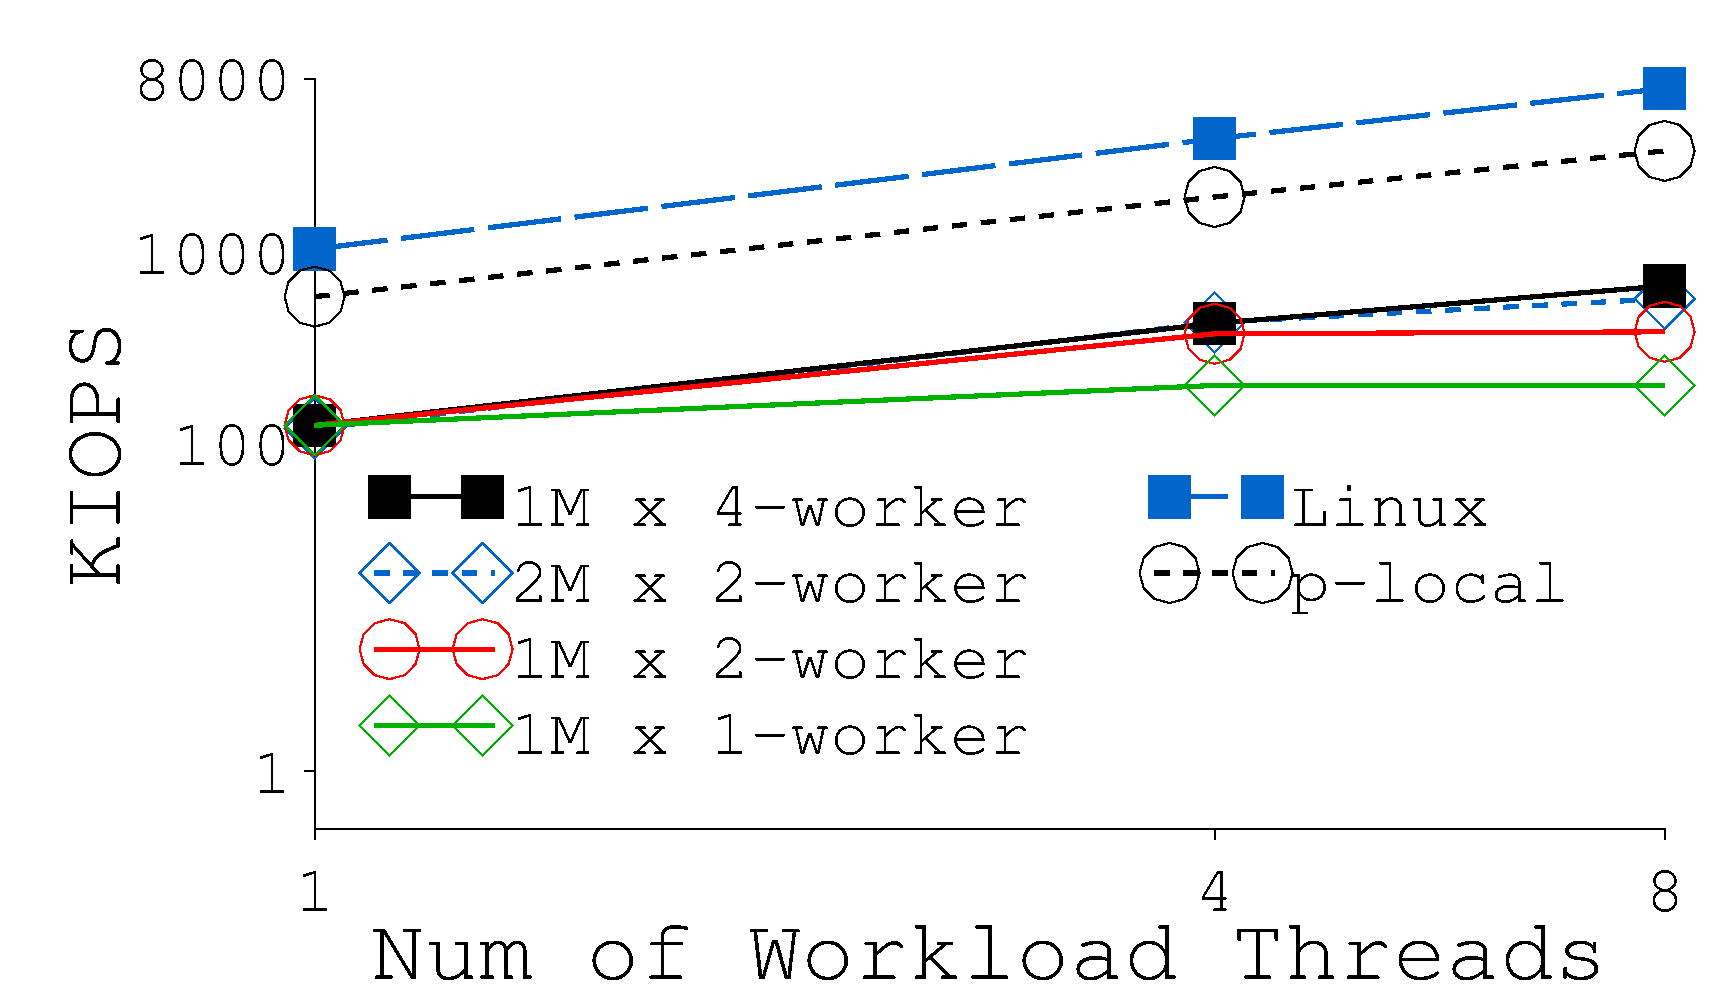
\includegraphics[width=0.5\textwidth]{lego/Figures/g_plot_LEGO_iops_memory.pdf}}
\caption[Memory Throughput]{Memory Throughput.}
\label{fig-iops-memory}
\end{center}
\end{figure*}
}
{
\begin{figure*}[th]
\begin{center}
\centerline{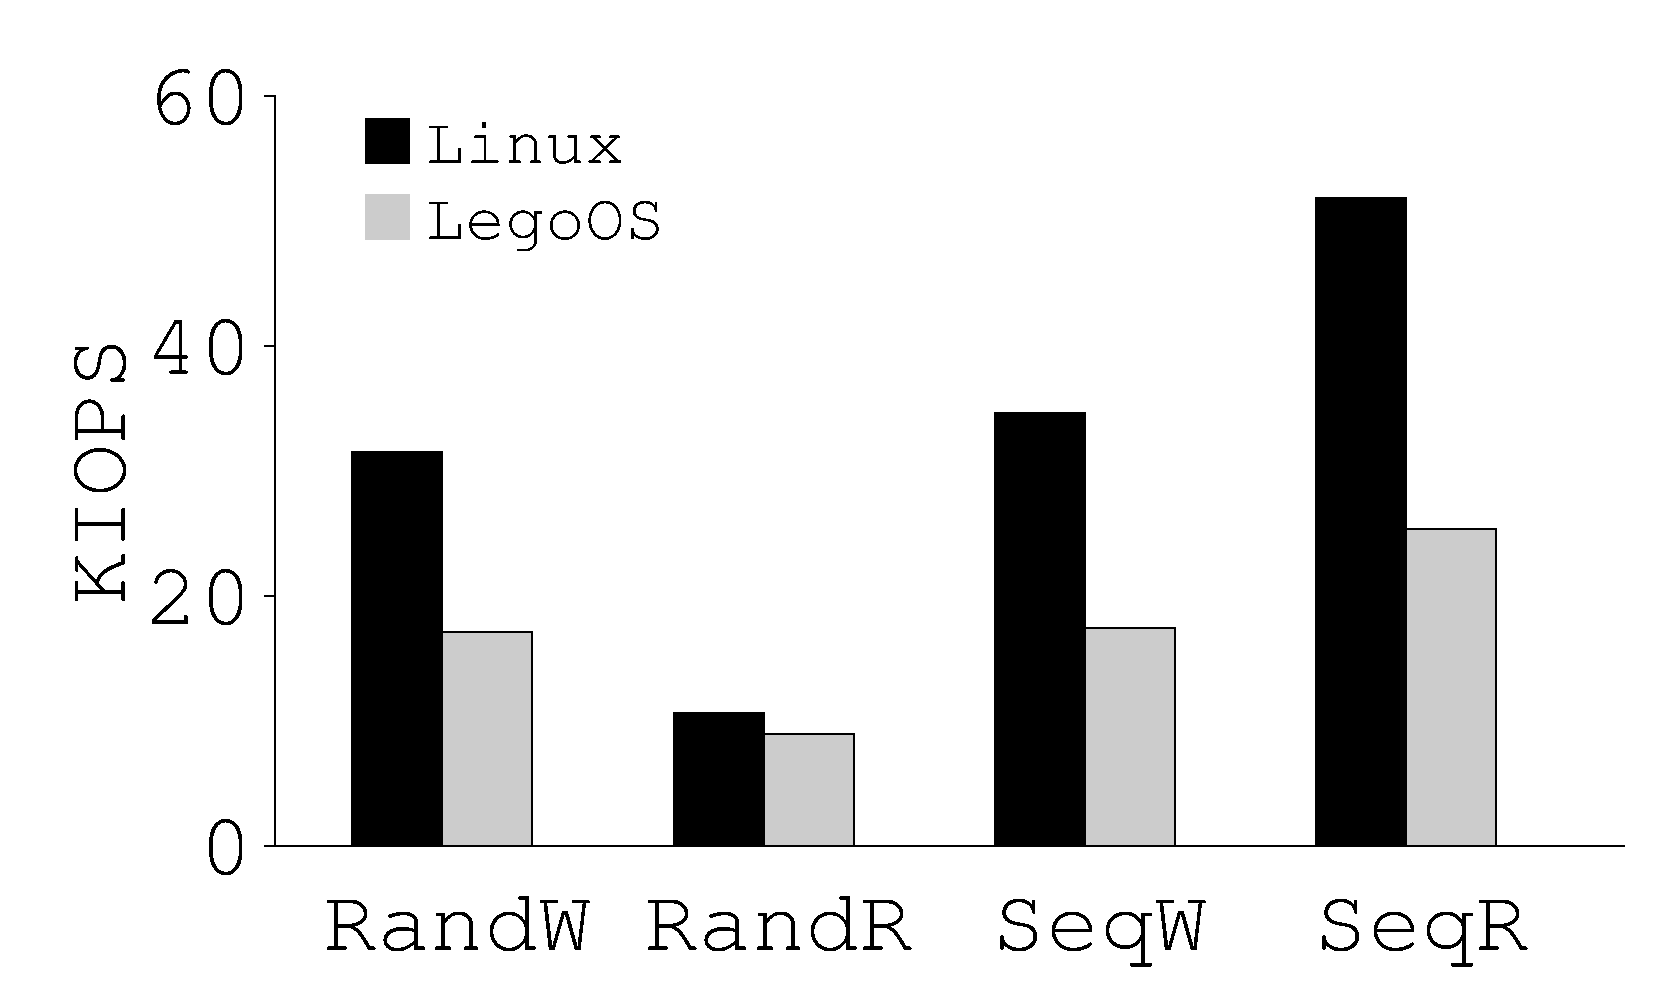
\includegraphics[width=0.5\textwidth]{lego/Figures/g_plot_LEGO_iops_storage.pdf}}
\caption[Storage Throughput.]{Storage Throughput.} 
\label{fig-iops-storage}
\end{center}
\end{figure*}
}
{
\begin{figure*}[th]
\begin{center}
\centerline{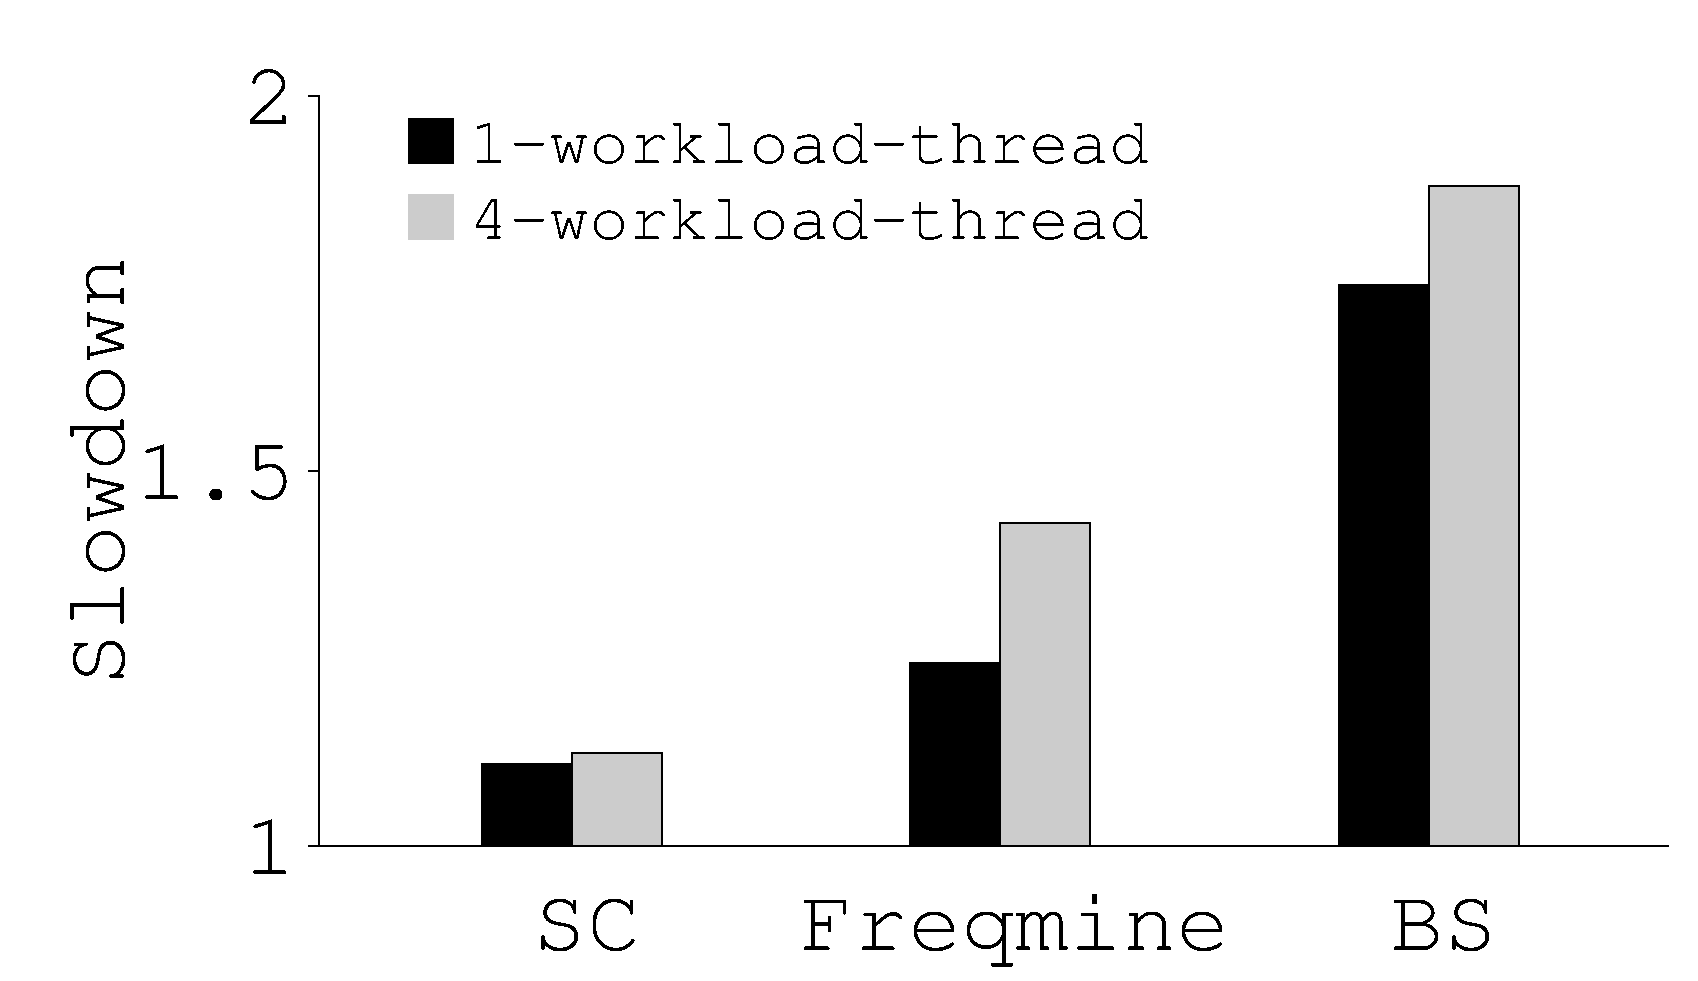
\includegraphics[width=0.5\textwidth]{lego/Figures/g_plot_LEGO_parsec.pdf}}
\caption[PARSEC Results.]{PARSEC Results. SC: StreamClsuter. BS: BlackScholes.}
\label{fig-parsec}
\end{center}
\end{figure*}
}
\subsection{Experience and Discussion}
We started our implementation of \lego\ from scratch to have a clean design and implementation that 
can fit the \splitkernel\ model
and to evaluate the efforts needed in building different \microos{}s.
However, with the vast amount and the complexity of drivers, we decided to port Linux drivers
instead of writing our own.
We then spent our engineering efforts on an ``as needed'' base
and took shortcuts by porting some of the Linux code. 
For example, we re-used common algorithms and data structures in Linux to easily port Linux drivers.
We believe that being able to support largely unmodified Linux drivers
will assist the adoption of \lego.
%For example, with our emulation of \lego\ hardware being x86 machines,
%we reused a lot of Linux's early boot code. 
%None of our components involve any hardware interrupts (all our network stacks use polling only)
%and we did not build any hardware interrupt handlers.

When we started building \lego, we had a clear goal of sticking to
the principle of ``clean separation of functionalities''.
However, we later found several places where performance could be improved 
if this principle is relaxed.
For example, for the optimization in \S\ref{sec:lego:zerofill} to work correctly,
\pcomponent\ needs to store the address range and permission for anonymous virtual memory regions --- 
memory-related information that otherwise only \mcomponent{}s need to know.
Another example is the implementation of \mremap.
With \lego' principle of \mcomponent{}s handling all memory address allocations,
memory \microos{}s will allocate new virtual memory address ranges for \mremap\ requests.
However, when data in the \mremap\ region is in \excache, 
\lego\ needs to move it to another set if the new virtual address does not fall into the 
current set.
If \mcomponent{}s are \excache-aware, they can choose the new virtual memory address
to fall into the same set as the current one.
Our strategy is to relax the clean-separation principle only by giving ``hints'', 
and only for frequently-accessed,
performance-critical operations.
